% textidote: ignore begin
\subsection{Components}\label{subsec:components}
% textidote: ignore end
The following Section will describe the most important models in the system.
This is done to give a better understanding of the architecture, more specifically the business logic.

As seen in Figure~\ref{fig:model-diagram}, the model describes the repository layer.
This layer connects both to the csv handler, but also the database as it uses the models to persist data.

\begin{figure}[H]
    \centering
    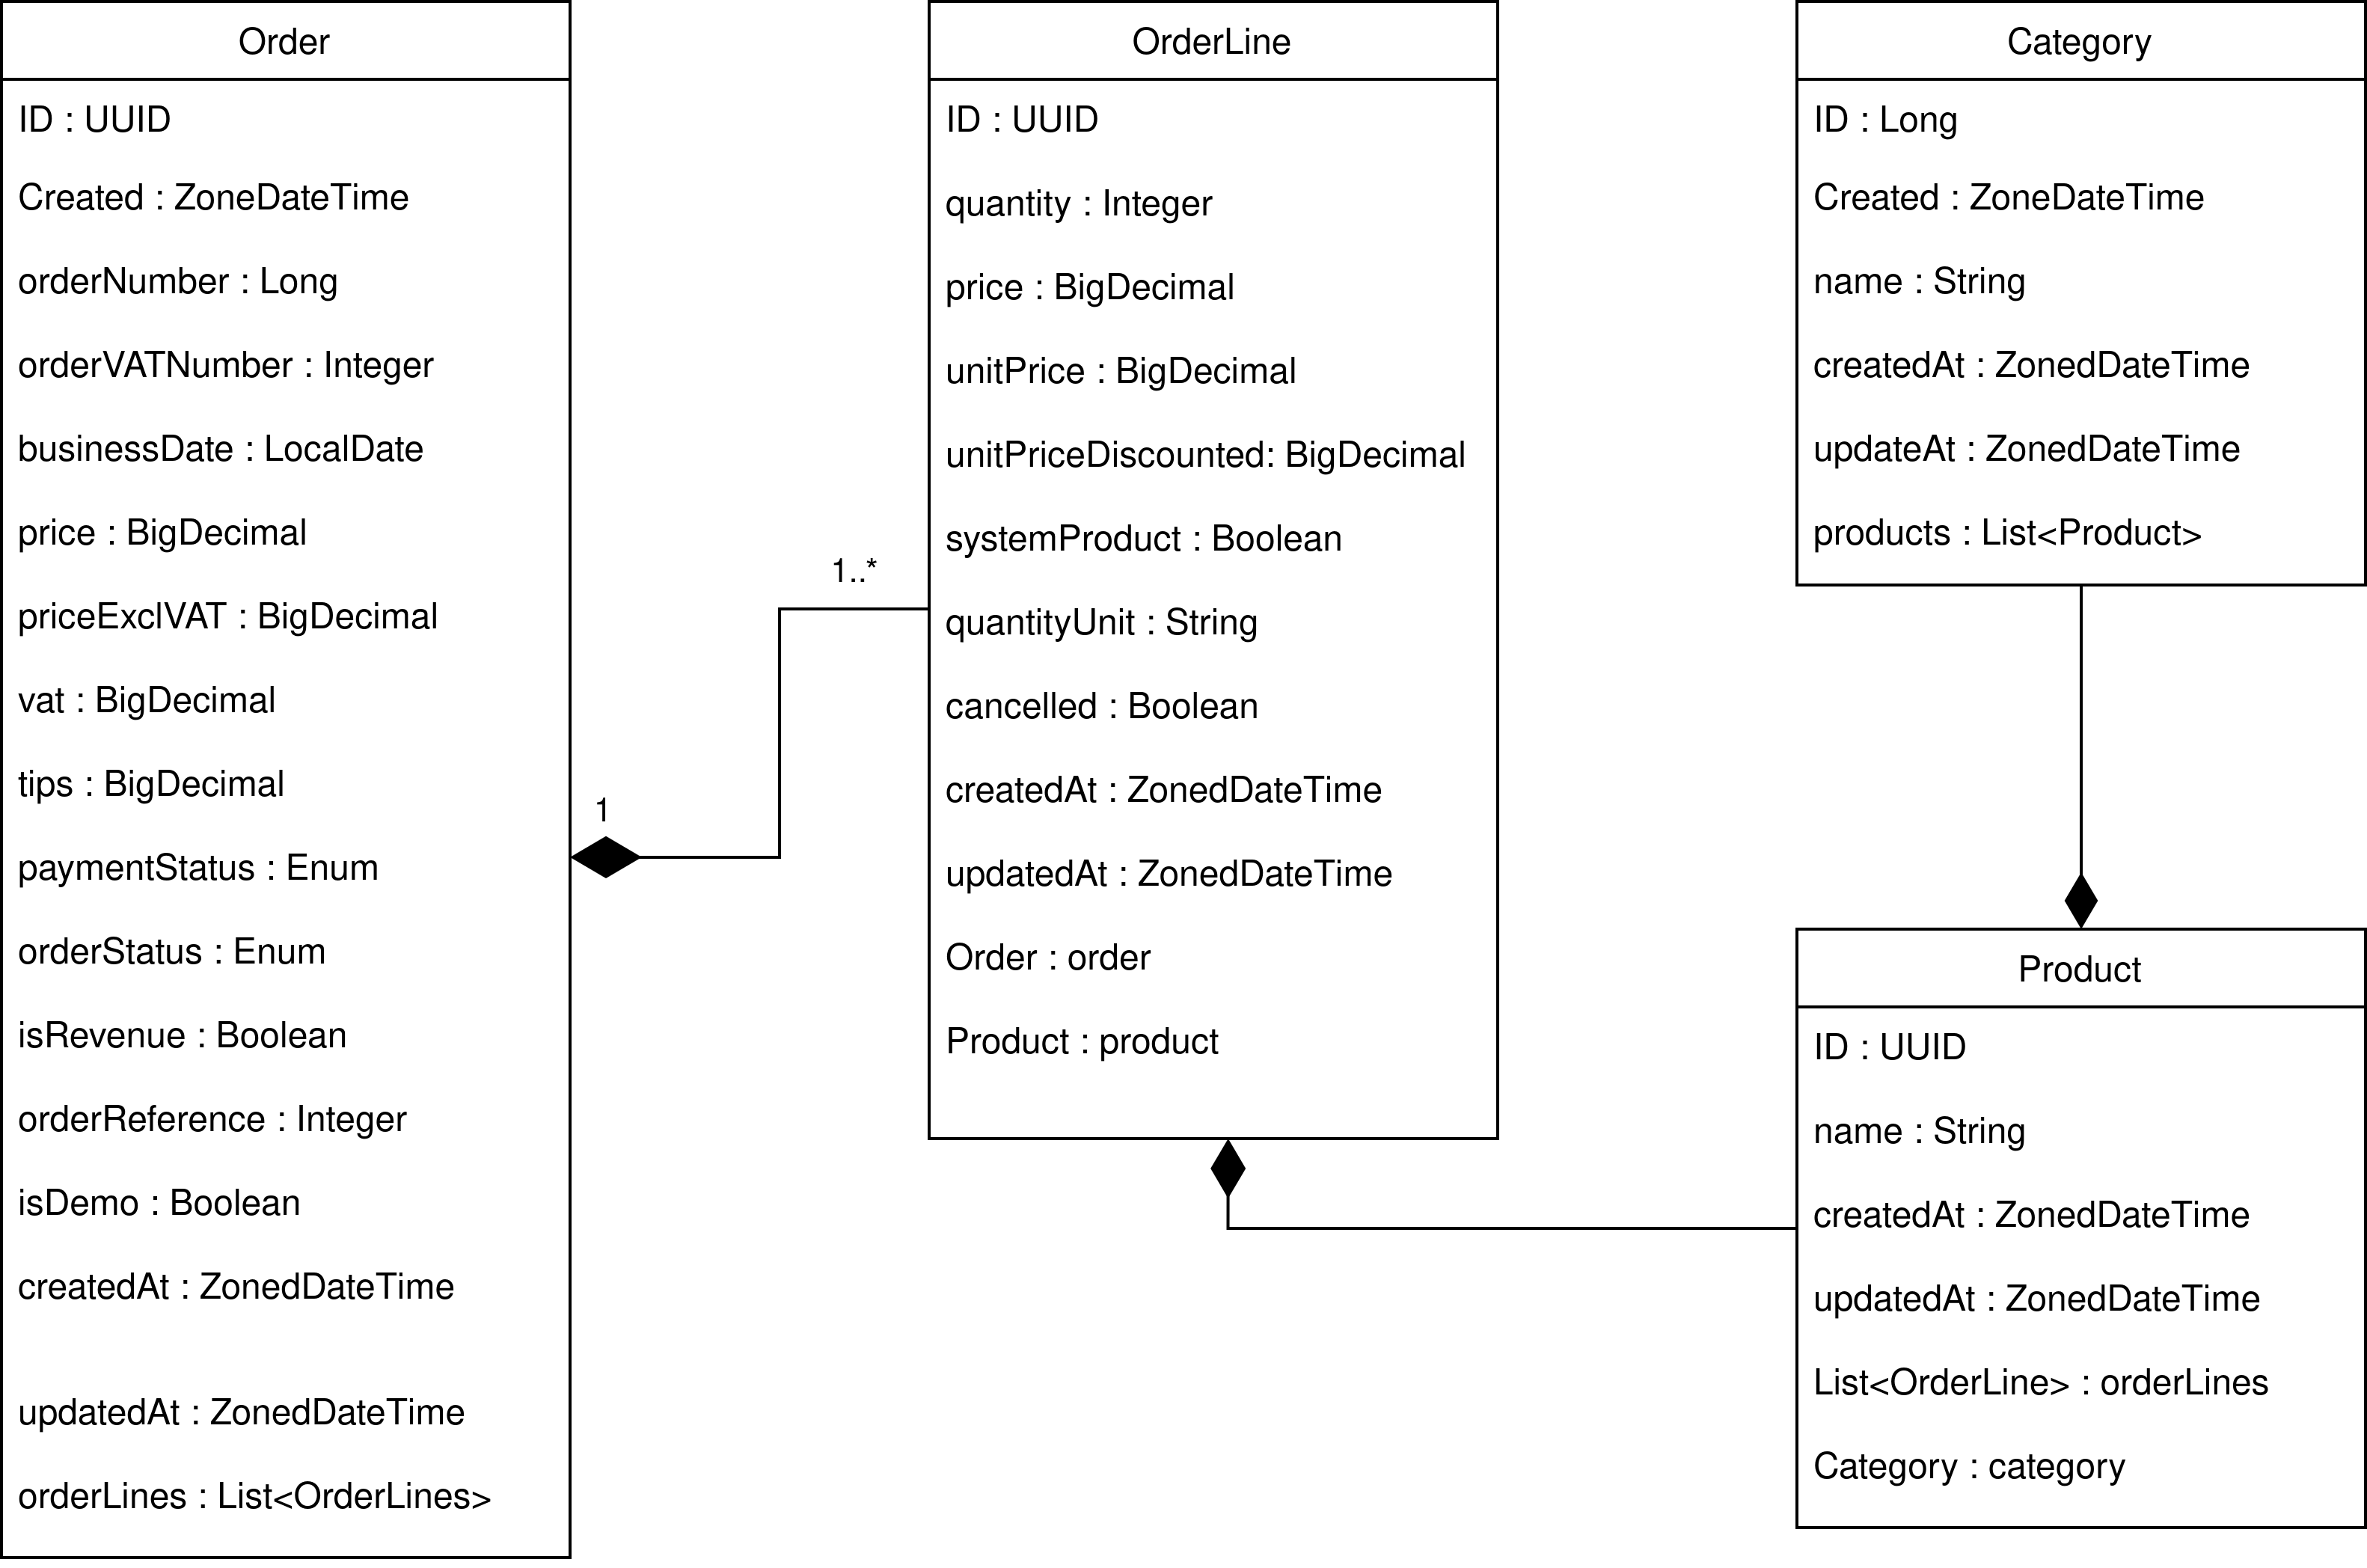
\includegraphics[width=0.7\textwidth]{model-diagram}
    \caption{Class diagram of the model, getter and setter methods are excluded.
    }\label{fig:model-diagram}
\end{figure}

